\pagebreak
\subsection{Passenger request}
\subsubsection{Scenarios}
\paragraph{Positive response}
Tom has already downloaded the mobile application called \textit{myTaxiService} and desires to request a taxi ride from his actual place, located in "Piazzale Gorini 18, Milano" to the "Stazione Centrale of Milano". He enters in the request section of its application, fills the form (source of the journey, number of passengers) and waits for a response from the service.
After a few seconds the system responds indicating that the taxi with identification code T345 is arriving at the requested address. The approximate waiting time for the taxi is 5 minutes.

\paragraph{Negative response}
Tom has already downloaded the mobile application called \textit{myTaxiService} and desires to request a taxi ride from his actual place, located in "Piazzale Gorini 18, Milano" to the "Stazione Centrale of Milano". He enters in the request section of its application, fills the form (source of the journey, number of passengers) and waits for a response from the service.
Immediately the system responds indicating that there are no taxi available in the corresponding zone and Tom is invited to retry later.

\subsubsection{Use case}
\begin{center}
\begin{longtable}{| p{.20\textwidth} | p{.80\textwidth} |} \hline
Use case & \textbf{Request a taxi} \\ \hline 
Actors & Passenger, Taxi Driver \\ \hline
Goals & A passenger must be able to request a taxi ride from a location he decides \\ \hline
Enter condition & \begin{itemize}
					\item The Passenger must already be registered to the service
					\item The Taxi driver must be registered to the service
					\item The Passenger must already have opened the application (mobile or web) and logged in
					\item The Taxi driver must be available
					\end{itemize} \\ \hline
Event flow & \begin{enumerate}
				\item The Passenger goes to the section for requesting a taxi ride
				\item \label{fillForm} The Passenger fills the form with:
				\begin{itemize}
					\item Meeting location
					\item Number of passengers
				\end{itemize}
				\item The Passenger submit the request to the system
				\item If there are missing data or the specified location is not valid or the number of passengers is greater than 3:
				\begin{enumerate}
					\item The system notifies the error to the Passenger
					\item Go back to Event flow \ref{fillForm}
				\end{enumerate}
				\item The request is stored in the system
				\item The system checks the location provided by the Passenger and computes the corresponding zone in the city
				\item The system, based on the city zone computed, retrieves the corresponding taxi queue
				\item If there are no taxi in the queue: \label{noTaxi}
				\begin{enumerate}
					\item Returns an error to the Passenger and invites him to retry later
					\item Go back to Event flow \ref{fillForm}
				\end{enumerate}
				\item The system takes the first taxi in the queue
				\item The system send the request to the taxi driver
				\item If the taxi driver does not accept the request:
				\begin{enumerate}
					\item The system puts the Taxi driver at the bottom of the queue
					\item Go back to Event flow \ref{noTaxi}
				\end{enumerate}
				\item The system sends to the Taxi driver the location of the meeting point with the Passenger
				\item The system computes an approximate waiting time for the Passenger
				\item The system informs the Passenger of the forthcoming arrival of the Taxi and the approximate waiting time.
			\end{enumerate} \\ \hline
Exit condition & The passenger is waiting for the taxi driver and the taxi driver is reaching him
\\ \hline
\caption{Use case: Taxi request from a Passenger}
\label{requestTaxiUC}
\end{longtable}

\end{center}
\subsubsection{Sequence diagrams}
\begin{figure}[H]
\centering
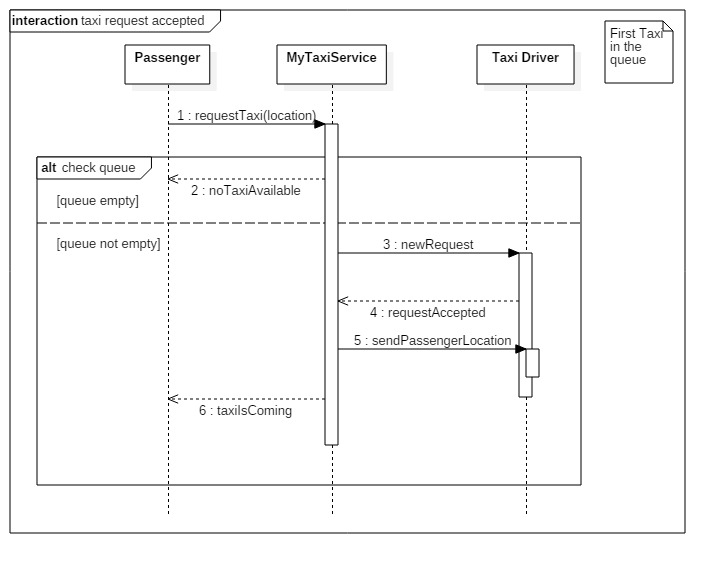
\includegraphics[scale=0.6]{Images/sequence_taxi_request_accepted}
\caption{An immediate positive response to the request of a Passenger}
\label{request_positive_TaxiSD}
\end{figure}

\begin{figure}[H]
\centering
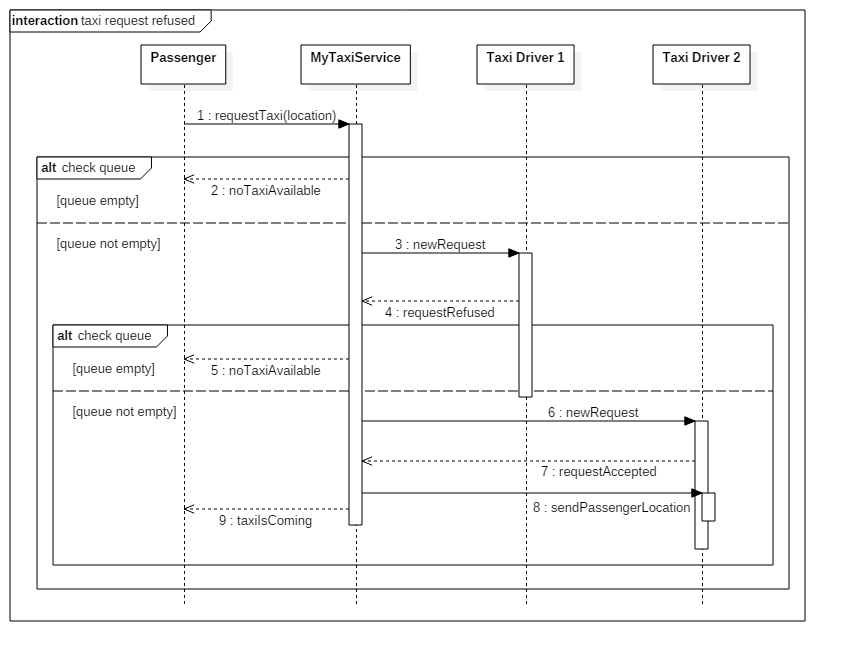
\includegraphics[scale=0.5]{Images/sequence_taxi_request_refused}
\caption{A complete positive response to the request of a Passenger}
\label{request_negative_TaxiSD}
\end{figure}


